% SEE GITHUB REPO AT https://github.com/gboeing/gis-bok-notebooks

\RequirePackage[l2tabu,orthodox]{nag}
\documentclass[11pt,letterpaper]{article}
\usepackage[T1]{fontenc}
\usepackage[utf8]{inputenc}
\usepackage{crimson}
\usepackage{helvet}
\usepackage[strict,autostyle]{csquotes}
\usepackage[USenglish]{babel}
\usepackage{microtype}
\usepackage{authblk}
\usepackage{booktabs}
\usepackage{caption}
\usepackage{endnotes}
\usepackage{geometry}
\usepackage{graphicx}
\usepackage{hyperref}
\usepackage{natbib}
\usepackage{rotating}
\usepackage{setspace}
\usepackage{titlesec}
\usepackage{url}

% location of figure files, via graphicx package
\graphicspath{{./figures/}}

% configure the page layout, via geometry package
\geometry{
	paper=letterpaper,
	top=4cm,
	bottom=4cm,
	left=4cm,
	right=4cm}
\setstretch{1.02}
\clubpenalty=10000
\widowpenalty=10000

% set section/subsection headings as the sans serif font
\titleformat{\section}{\normalfont\sffamily\large\bfseries}{\thesection.}{0.3em}{}
\titleformat{\subsection}{\normalfont\sffamily\small\bfseries}{\thesubsection.}{0.3em}{}

% make figure/table captions sans-serif small font
\captionsetup{font={footnotesize,sf},labelfont=bf,labelsep=period}

% configure pdf metadata and link handling
\hypersetup{
	pdfauthor={Geoff Boeing and Daniel Arribas-Bel},
	pdftitle={GIS and Computational Notebooks},
	pdfsubject={GIS and Computational Notebooks},
	pdfkeywords={GIS,},
	pdffitwindow=true,
	breaklinks=true,
	colorlinks=false,
	pdfborder={0 0 0}}

\title{GIS and Computational Notebooks}
\author{Geoff Boeing and Daniel Arribas-Bel}
\date{2020}

\begin{document}

\maketitle

\begin{abstract}
Nunc efficitur dui non elementum tincidunt. Sed eget ultricies dui, nec congue massa. Fusce at faucibus arcu, a dapibus leo. Donec congue viverra lorem, et viverra massa pellentesque eu. Mauris dictum efficitur lectus, nec tempus velit viverra at. Pellentesque habitant morbi tristique senectus et netus et malesuada fames ac turpis egestas. In tristique urna purus, a viverra sapien vehicula at. Donec id lectus dui. Class aptent taciti sociosqu ad litora torquent per conubia nostra, per inceptos himenaeos. Ut viverra leo ac velit aliquam, id pellentesque est maximus. Proin laoreet aliquet ex vel semper. Integer congue sollicitudin elit, ut tincidunt odio tincidunt quis. Duis eu mi sed massa pellentesque efficitur.
%\vspace{1cm}
\end{abstract}

\section*{Definitions}

5-7 definitions of key terms, TBD after first draft

Computational notebook

Jupyter

\section{Introduction}

A computational notebook is a computer file that contains code, output, images, and narrative text woven together. Notebooks allow users to consolidate their analytics workflow code, documentation, and results into a single reproducible and distributable package. They also enable interactive computing in the literate programming paradigm. This chapter introduces these concepts, positions computational notebooks as a key emerging tool in the GIS landscape, and discusses their value for geospatial analysts.

The notebook interface was developed in the 1980s by Mathematica as a closed-source commercial tool for scientists \citep{somers_scientific_2018}. During the 2010s, open-source notebook development, spearheaded by Project Jupyter, expanded throughout research and practice by supporting popular languages in the open-source and open-science communities such as Python, R, and Julia. Today many geospatial scholars and practitioners use notebooks to load, clean, filter, analyze, visualize, and model spatial data.

Recent years have witnessed rapid adoption of computational notebooks, particularly Jupyter notebooks, among data scientists and instructors across disciplines like biology, astronomy, economics, and geography \citep{perkel_why_2018}. To understand this shift, we must consider notebooks' capabilities and the value they create for analysts, researchers, teachers, and students.

\section{How Computational Notebooks Work}

\subsection{The Paradigm}

Scientific researchers and analysts historically used lab notebooks to record their workflow's questions, hypotheses, data, models, results, and all the various analytical decisions made along the way. This was important for organizing research activities and documenting all the \enquote{whats,} \enquote{whys,} and \enquote{hows} of the serpentine scientific process for subsequent recollection and replication. Computational notebooks mimic these traditional lab notebooks digitally and enhance them through two paradigms: literate programming and interactive scientific computing.

To explain these paradigms, let us contrast them with a traditional computer program which consists of lines of code and optional inline comments and is executed linearly from beginning to end. In literate programming, a computer program instead consists of both code and natural language narratives woven together to explain and document the logic of the program \citep{knuth_literate_1992}. In interactive scientific computing, a computer program interacts in real-time with its user and these interactions shape its execution flow \citep{perez_ipython:_2007}.

Thus, while a traditional program runs through its code linearly, a computational notebook can be executed nonlinearly and include natural language narratives documenting and explaining each chunk of code alongside its results and output.

\begin{figure*}[tbp]
	\centering
	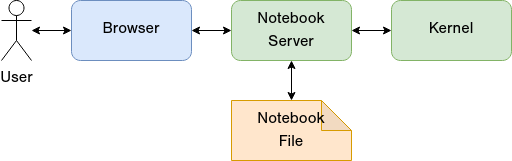
\includegraphics[width=0.8\textwidth]{notebook-architecture.png}
	\caption{The architecture of a Jupyter notebook.}
	\label{fig:notebook_architecture}
\end{figure*}

\subsection{Notebook Architecture}

Many different kinds of computational notebooks exist today for many different programming languages, but all of these various implementations share a set of common features. As the Jupyter notebook has become by far the most prominent, we will focus our discussion on it as an illustrative example.

The architecture of a Jupyter notebook comprises four components: a web browser, a notebook server, a notebook file, and a kernel \citep{kluyver_jupyter_2016}. As illustrated in Figure \ref{fig:notebook_architecture}, the web browser visits the URL of the notebook server, which reads the notebook file and sends it to the browser. The browser renders the notebook as a web page with individual cells in which the user can type code or text.

When the user executes a code cell, the browser sends that code to the server, which passes it to the kernel, a back-end interpreter which runs the code and returns the result to the browser via the notebook server. The browser renders this result inline in the notebook beneath the code cell. Thus, computational output such as individual calculations, tables, or figures appears beside the code that generated it.

Notebook kernels are language-specific. Hundreds of Jupyter kernels exist for dozens of different programming languages. The most popular languages for data science are all supported, including Python, R, and Julia.

\begin{figure*}[tbp]
	\centering
	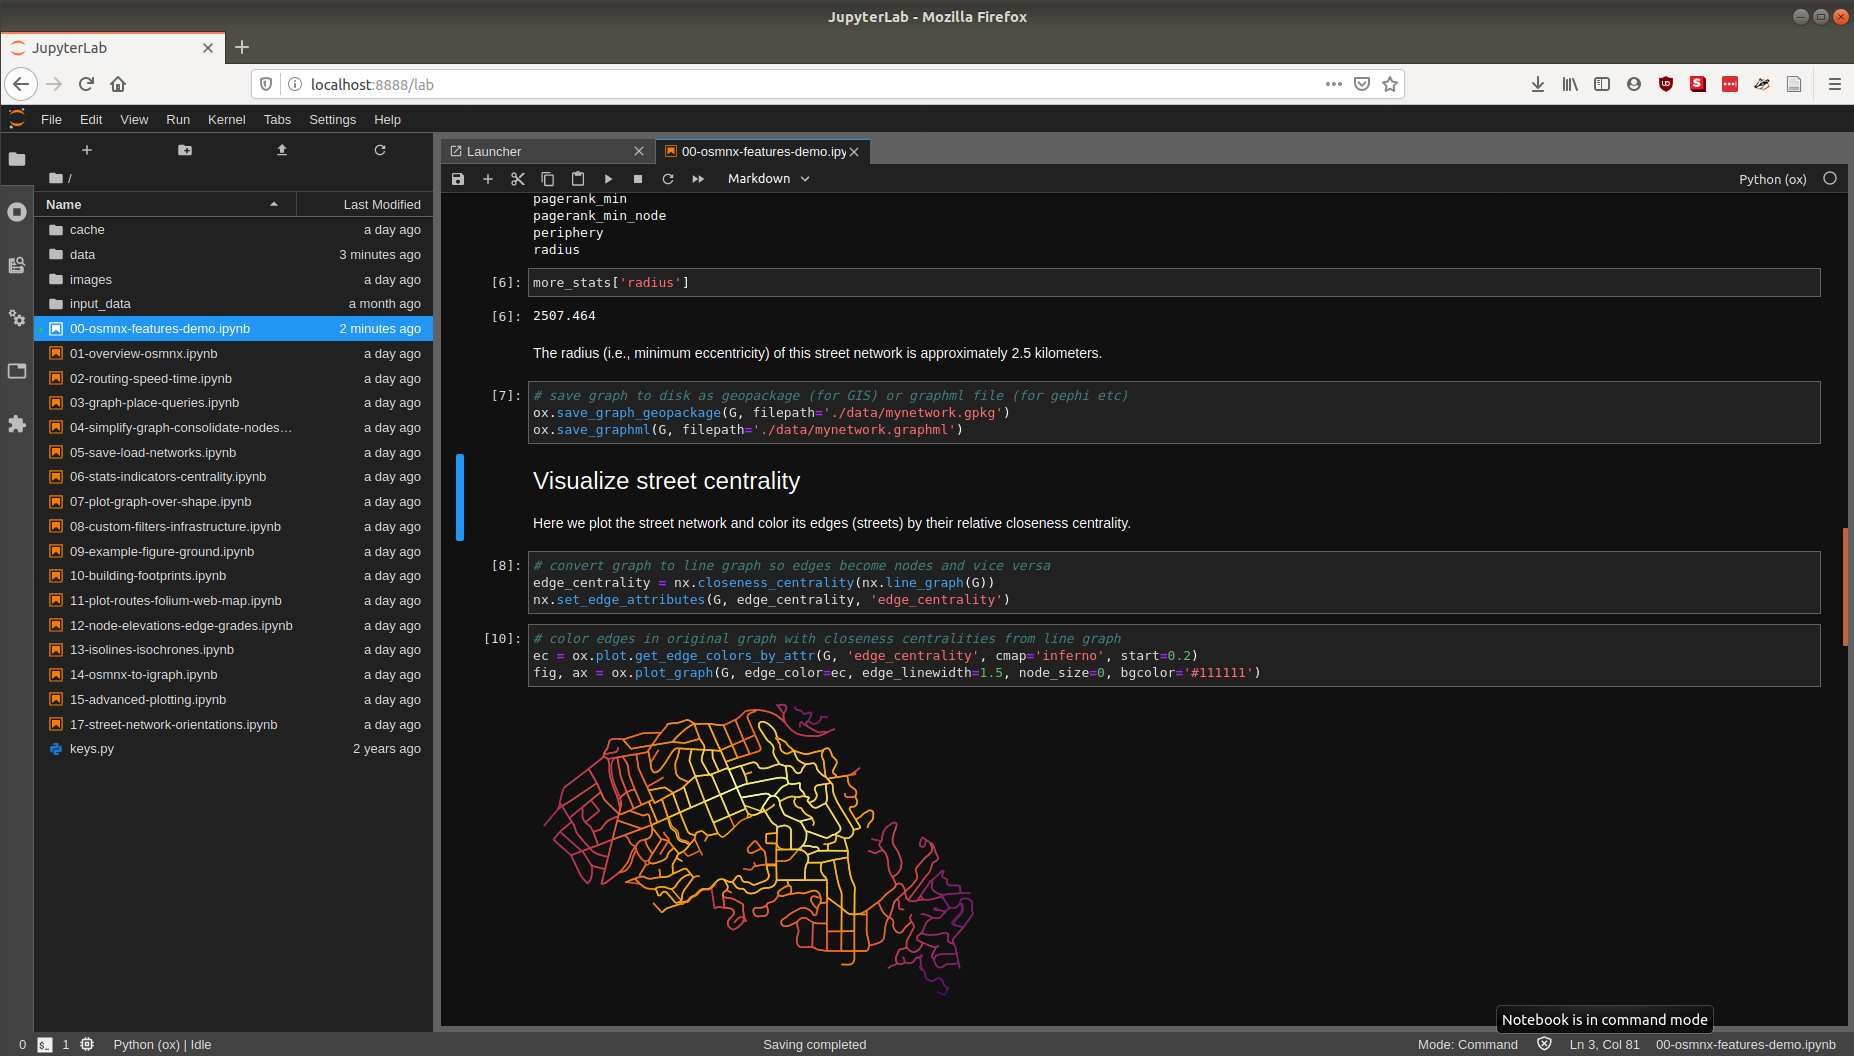
\includegraphics[width=1\textwidth]{jupyterlab-interface.png}
	\caption{The JupyterLab notebook interface.}
	\label{fig:jupyterlab_interface}
\end{figure*}

\subsection{Notebook Usage}

As discussed briefly above, a web browser renders the user interface of the computational notebook. In the Jupyter ecosystem, this user interface is called JupyterLab.

JupyterLab shares many common user interface elements with other computational notebooks. It primarily consists of a main work area and a sidebar to browse files and running kernels, as illustrated in Figure \ref{fig:jupyterlab_interface}. The main work area contains the currently open notebooks. Here, notebooks can be created, edited, and executed. Users can add or remove notebook cells, move cells around to reorder them, type code or markdown text into cells, or run one or more cells. Given the interactive paradigm, a cell or cells can be run once or many times repeatedly, and cells may be run in any order the user desires. Due to this possibly nonlinear flow of execution, it is important to periodically restart the kernel and run all cells to ensure that objects are defined and used in the expected order of operations.

Computational notebooks are increasingly used today in pedagogy, research, and practice. Instructors use them to introduce students to coding and data science because they can show the results of each computation, step by step, and explain each new language detail along the way \citep{reades_teaching_2020}. Researchers use them to document, explain, and visualize their research questions, hypotheses, data, experiments, and results inline with the code \citep{perkel_why_2018}. Software developers use them to provide visual, narrative usage examples and demonstrations of their software packages for newcomers to learn how they work \citep{boeing_urban_2020}. All of a computational notebook's code, text, and multimedia content is stored in a single notebook file, so they can easily be shared and distributed and they work well in collaborative version control systems.

\section{GIS in a Computational Notebook}

>> DANI
(ca. 750w)
Why Notebooks for GIS?
\enquote{If they didn't exist we'd have to invent them}
Computational nature of modern gis: this is becoming more and more important
Cleaning as central to modern gis
Expose the nitty gritty details to make analysis decisions explicit

\section{Notebooks Are Not Enough}

>> DANI
(ca. 500w)
Standing on the shoulders of giants: notebooks are not enough
Open source ecosystem
Transferrable platforms/environments/containers -> isolate what you need for reproducibility

\section{Notebooks in Action}

Today, the geographic data science ecosystem is most robust in R (particularly the r-spatial community) and especially Python where many packages exist to support spatial analysis and modeling such as geopandas (geospatial data wrangling and analysis), PySAL (advanced spatial analysis and econometrics), matplotlib (data visualization), OSMnx (street networking modeling and analytics),  cartopy (mapping), folium (web mapping), and many more. These tools allow data scientists to completely replace legacy desktop GIS software with reproducible, universal analytics workflows in computational notebooks.

\begin{figure*}[htb]
	\centering
	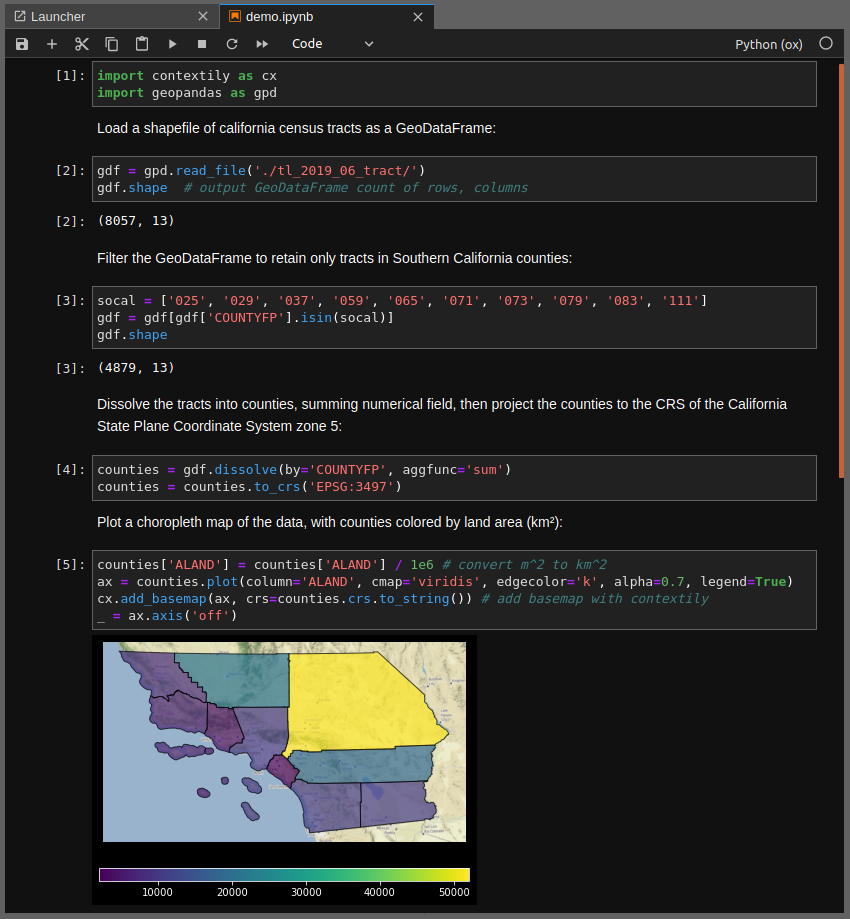
\includegraphics[width=0.8\textwidth]{code-demo.png}
	\caption{Simple real-world usage example that demonstrates basic GIS in a computational notebook, using JupyterLab and Python.}
	\label{fig:code_demo}
\end{figure*}

We conclude this chapter with a real-world usage example using JupyterLab and Python that demonstrates the absolute basics of doing GIS in a computational notebook, illustrated in Figure \ref{fig:code_demo}. In cell 1, we import the geopandas package for geospatial data handling and give it the friendly standard \enquote{gpd} handle. In cell 2, we use geopandas to read an ESRI shapefile containing all the census tracts in California, turn it into a GeoDataFrame, and output the shape of the resulting GeoDataFrame. We have 8,057 rows (i.e., census tracts) and 13 columns (i.e., variables). In cell 3, we create a list of all the county IDs in Southern California, then filter the GeoDataFrame to only retain tracts whose county IDs appear in that list. Outputting the shape of the resulting GeoDataFrame here reveals that we have retained only 4,879 of the original 8,057 tracts.

In cell 4, we dissolve and project the GeoDataFrame. First we aggregate the tracts up to the county level with a standard spatial dissolve operation and sum their numerical attributes to get new county totals. Then we project the GeoDataFrame from its original coordinate reference system (as defined in the shapefile) to a new one representing the meter-based California State Plane Coordinate System zone 5. Finally, in cell 5, we convert the land area column from m\textsuperscript{2} to km\textsuperscript{2}, then plot a (very basic) choropleth map of the spatial data, with counties colored by land area. This notebook can be executed linearly like a script by running it from the top-down, or it can be executed nonlinearly by a user choosing individual cells to run one or multiple times in an arbitrary order.

\setlength{\bibsep}{0.00cm plus 0.05cm}
\bibliographystyle{apalike}
\bibliography{GIS-BoK}

\section*{Learning Objectives}

TBD after first draft

\section*{Instructional Assessment Questions}

TBD after first draft

\section*{Additional Resources}

TBD after first draft

should include Dani's GDS course resources

\section*{Associated Image}

Figure \ref{fig:jupyterlab_interface} can be used as the associated image.

\end{document}
